\documentclass[10pt,a4paper]{article}
\usepackage[margin=2cm]{geometry}
\usepackage{amsmath,amssymb,booktabs,graphicx,caption,subcaption,xcolor,float,hyperref,tikz}
\usetikzlibrary{arrows.meta,positioning,calc}
\hypersetup{colorlinks=true,linkcolor=blue!50!black,urlcolor=blue!50!black}
\captionsetup{font=small,labelfont=bf}
\newcounter{diagram}
\newcommand{\diagramcaption}[1]{\refstepcounter{diagram}\par\smallskip\noindent{\small\textbf{Diagram~\thediagram.} #1}}
\title{\vspace{-1.2cm}\textbf{Without rounds, a swarm holds its proof less firmly}\\[2pt]
\large Simulation 2 (asynchronous activation), setup \texttt{task003-symmetric}: first results}
\author{LLM-free simulator, runs of 9 October 2026}
\date{}
\begin{document}
\maketitle
\vspace{-1cm}

\paragraph{Summary.} The 24 agents together hold a proof of allocation A0 (the truth).
Simulation 2 removes the day/night rounds of Simulation 1: agents and the controller act at
random times, remembered facts fade continuously, and the shared board fades too. When
agents forget, \textbf{the swarm holds its own proof less firmly} than in Simulation 1, and
\textbf{the false controller is weaker} (gain 0.13 against 0.22). How fast the controller
acts matters little for where the swarm ends up, but \textbf{fast controllers overshoot and
then relax}. Turning the vote gate off doubles the truth controller's gain at six times
the messages. As in Simulation 1, help with the truth \textbf{replaces the agents' own
proofs}. Effects persist for ten time units after the controller stops. Main hypotheses
were confirmed on a second, independent set of random draws.

\section{Setup}

\begin{center}
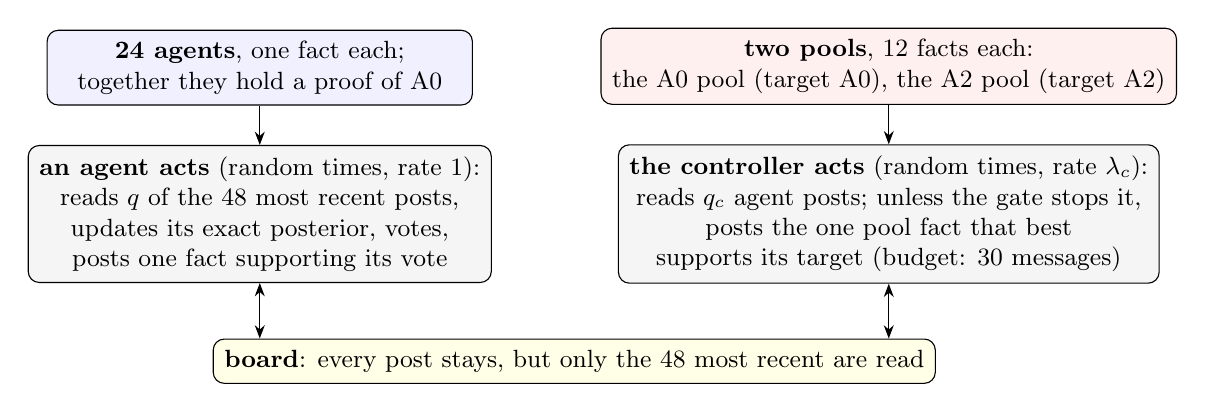
\begin{tikzpicture}[font=\small, box/.style={draw, rounded corners, align=center, inner sep=4pt}]
  \node[box, fill=gray!8, minimum width=5.4cm] (agent) {\textbf{an agent acts} (random times, rate 1):\\
     reads $q$ of the 48 most recent posts,\\ updates its exact posterior, votes,\\ posts one fact supporting its vote};
  \node[box, fill=gray!8, right=1.6cm of agent, minimum width=5.4cm] (ctrl) {\textbf{the controller acts} (random times, rate $\lambda_c$):\\
     reads $q_c$ agent posts; unless the gate stops it,\\ posts the one pool fact that best\\ supports its target (budget: 30 messages)};
  \node[box, fill=blue!6, above=0.5cm of agent, minimum width=5.4cm] (agents) {\textbf{24 agents}, one fact each;\\
     together they hold a proof of A0};
  \node[box, fill=red!6, above=0.5cm of ctrl, minimum width=5.4cm] (pool) {\textbf{two pools}, 12 facts each:\\
     the A0 pool (target A0), the A2 pool (target A2)};
  \coordinate (mid) at ($(agent.south)!0.5!(ctrl.south)$);
  \node[box, fill=yellow!10, anchor=north, minimum width=8cm] (board) at ($(mid)+(0,-0.7)$) {\textbf{board}: every post stays, but only the 48 most recent are read};
  \draw[-{Stealth}] (agents) -- (agent);
  \draw[-{Stealth}] (pool) -- (ctrl);
  \draw[{Stealth}-{Stealth}] (agent.south) -- (agent.south |- board.north);
  \draw[{Stealth}-{Stealth}] (ctrl.south) -- (ctrl.south |- board.north);
\end{tikzpicture}
\diagramcaption{Simulation 2. There are no rounds. Each remembered fact is forgotten after a
random lifetime (on average a fraction $\rho$ survives one time unit) and comes back if read
again. The controller acts for $0 \le t < 30$; agents continue alone until $t = 40$.}
\end{center}

\noindent Agents are exact Bayesian reasoners. An agent's vote is drawn from its posterior
(probability matching). The \emph{vote gate} keeps the controller silent when at least 75\%
of the posts it read come from agents who voted for its target; the \emph{proof stop} keeps
it silent when what it read already proves its target. The grid: posts read
$q \in \{3,6,12\}$, $q_c \in \{3,6,12,24\}$, memory $\rho \in \{0.75, 1\}$, controller rate
$\lambda_c \in \{0.5,1,2,4,8\}$ actions per time unit, gate on/off, proof stop on/off;
1{,}000 episodes per setting. Control is measured by the \emph{gain}
\begin{equation}\label{eq:gain}
G(t) = \frac{1}{E}\sum_{e=1}^{E}\Bigl[m_{\text{target}}(t)^{\text{ctrl}}(e) - m_{\text{target}}(t)^{\text{silent}}(e)\Bigr],
\end{equation}
where $m_k(t)$ is the agents' mean belief in allocation $k$ and each episode $e$ uses the same
random draws with and without the controller. Unless stated otherwise: $q = 6$, $q_c = 12$,
$\rho = 0.75$, gate on, proof stop on.

\section{Without a controller: the proof is held less firmly}

\begin{figure}[H]
\centering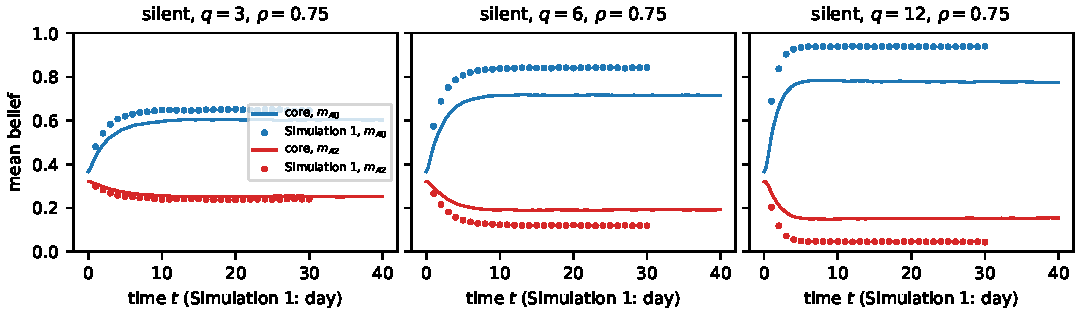
\includegraphics[width=0.95\linewidth]{figures/fig_silent.pdf}
\caption{Silent swarm, $\rho = 0.75$: mean belief in A0 (blue) and A2 (red) over time.
Dots: Simulation 1, end of each day. Lines: Simulation 2.}
\label{fig:silent}
\end{figure}

With forgetting, the silent swarm settles at a lower belief in the truth than in
Simulation 1: $m_{\text{A0}}(30) = 0.60 / 0.72 / 0.78$ against $0.65 / 0.84 / 0.94$ for
$q = 3 / 6 / 12$ (Figure~\ref{fig:silent}); confirmed with fresh random draws ($-0.12$ at
$q = 6$). In Simulation 1 memories change only at dawn, and every agent acts right after a
full day of new posts. Here facts expire at random moments between an agent's actions, so
fewer facts are held together at any time and complete proofs are rarer. With full memory
($\rho = 1$) both simulations end with every agent proving A0, and no controller can change
that: all gains at $\rho = 1$ are zero.

\section{Control}

\begin{figure}[H]
\centering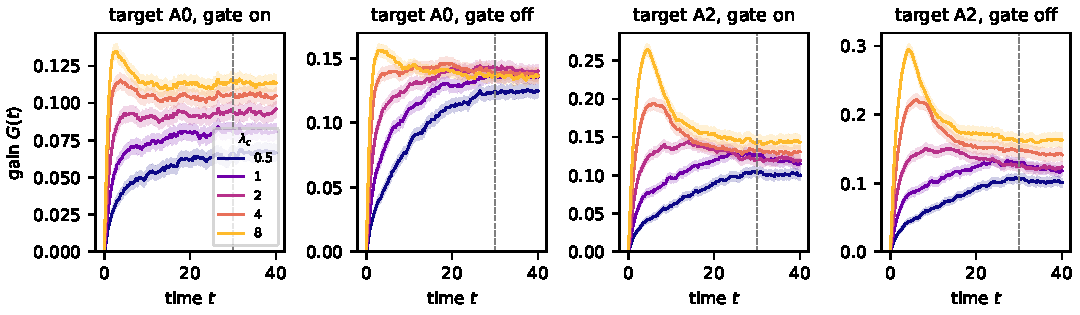
\includegraphics[width=0.98\linewidth]{figures/fig_gain_time.pdf}
\caption{Gain over time, Eq.~(\ref{eq:gain}), by controller rate $\lambda_c$; the controller
stops at $t = 30$ (dashed). Bands: 95\% intervals.}
\label{fig:gaintime}
\end{figure}

\begin{figure}[H]
\centering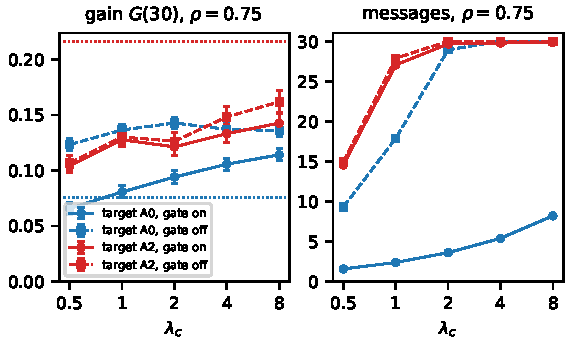
\includegraphics[width=0.62\linewidth]{figures/fig_rate.pdf}
\caption{Left: gain at $t = 30$ against the controller rate (target A0 blue, A2 red; gate on
solid, off dashed; dotted: Simulation 1 with one fact per night). Right: messages sent per
episode (budget 30).}
\label{fig:rate}
\end{figure}

\begin{itemize}\itemsep1pt
\item \textbf{The false controller is weaker than in Simulation 1}: $G(30) = 0.13$ against
  $0.22$ (one fact per night in Simulation 1); confirmed with fresh draws ($-0.09$). The
  truth controller is unchanged ($0.08$ in both).
\item \textbf{The rate changes the path more than the end point}
  (Figures~\ref{fig:gaintime}, \ref{fig:rate}). From $\lambda_c = 0.5$ to $8$ the gain at
  $t = 30$ rises from $0.10$ to $0.14$ (target A2) and from $0.07$ to $0.11$ (target A0).
  A fast controller spends its budget within a few time units, its gain peaks early and
  then relaxes: target A2 at $\lambda_c = 8$ peaks at $0.26$ ($t \approx 4.5$) and falls to
  $0.14$.
\item \textbf{The effect persists}: ten time units after the controller stops, the gain has
  changed by at most $0.021$ in every setting, less than one agent's worth of belief
  ($1/24 \approx 0.042$); confirmed with fresh draws.
\end{itemize}

\begin{figure}[H]
\centering
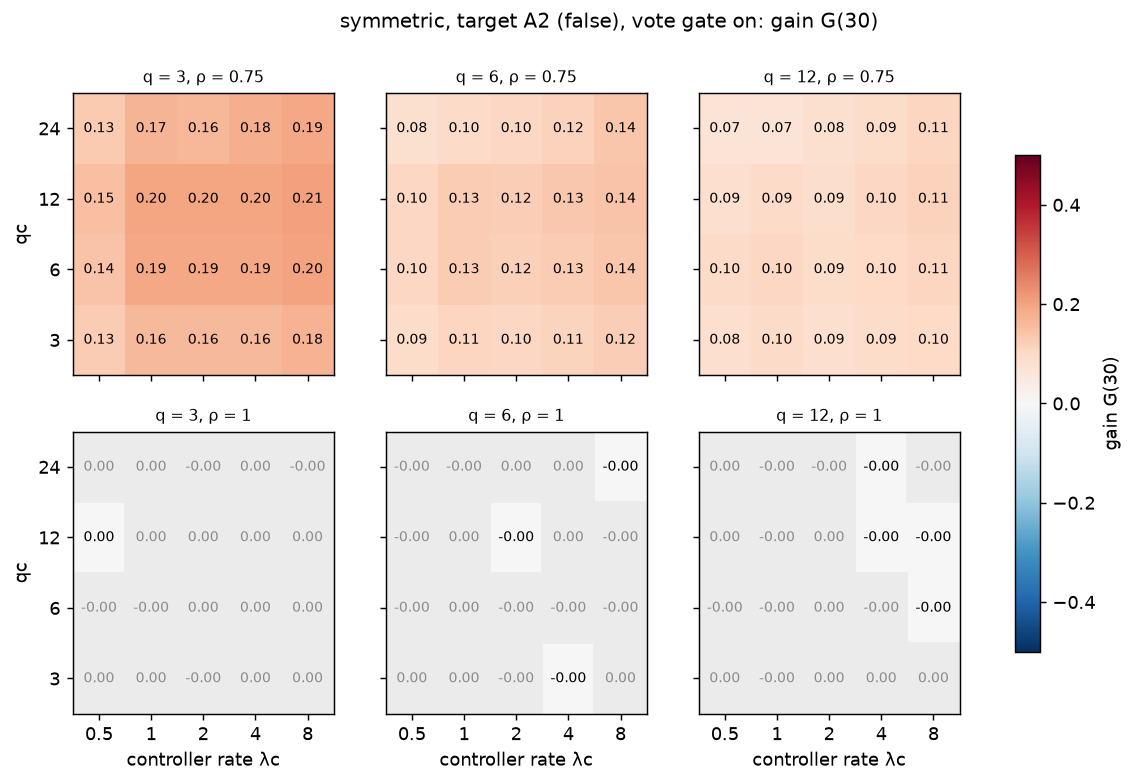
\includegraphics[width=0.72\linewidth]{figures/phase_false_gateon.png}\\[2pt]
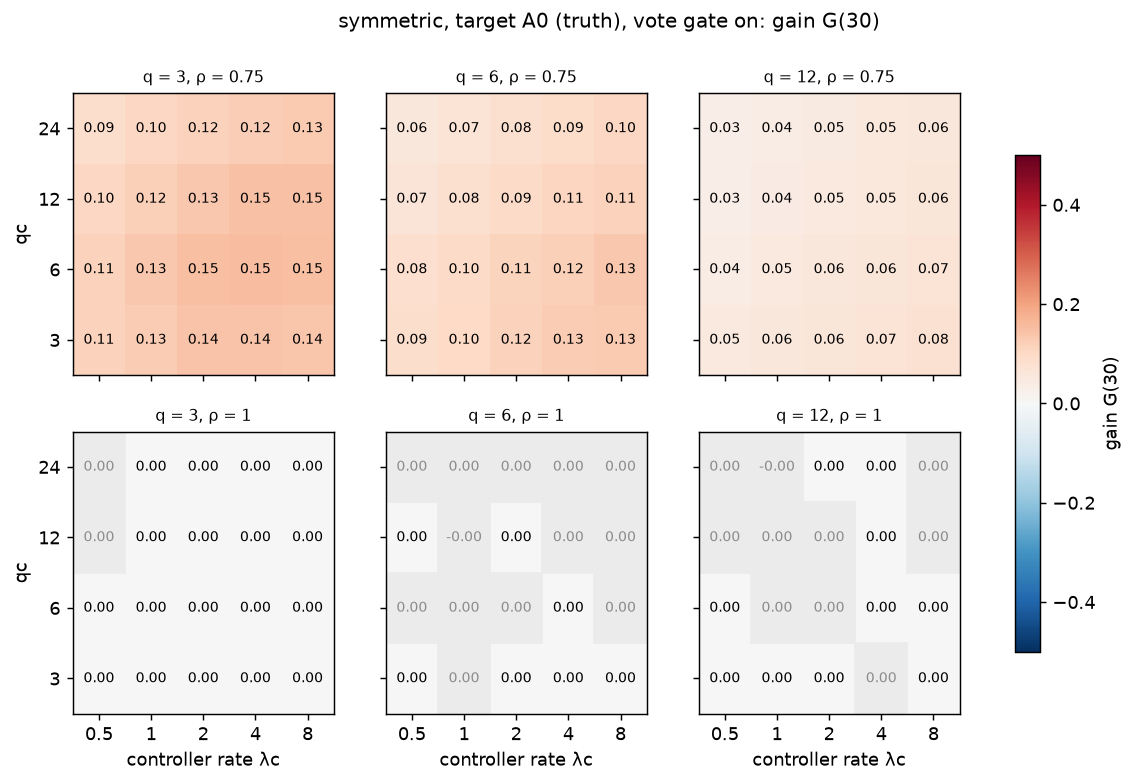
\includegraphics[width=0.72\linewidth]{figures/phase_truth_gateon.png}
\caption{Gain $G(30)$ over controller rate (x) and posts read by the controller $q_c$ (y),
for every $q$ (columns) and $\rho$ (rows); gate on. Top: target A2; bottom: target A0.
Grey numbers: 95\% interval includes 0.}
\label{fig:phase}
\end{figure}

\section{The vote gate and the proof stop}

The false controller is almost never stopped by the gate (the A2 share rarely reaches 75\%),
so turning the gate off changes nothing for it. The truth controller often is: with the gate
off it sends about six times as many messages (9.3 against 1.6 at $\lambda_c = 0.5$) and its
gain roughly doubles ($0.066 \to 0.123$; $+0.055$ at $\lambda_c = 1$, confirmed with fresh
draws). The proof stop has no effect larger than one agent's worth of belief ($1/24$) in any
setting, and turning it off costs up to 25 extra messages per episode.

\section{Help with the truth replaces the agents' own proofs}

\begin{figure}[H]
\centering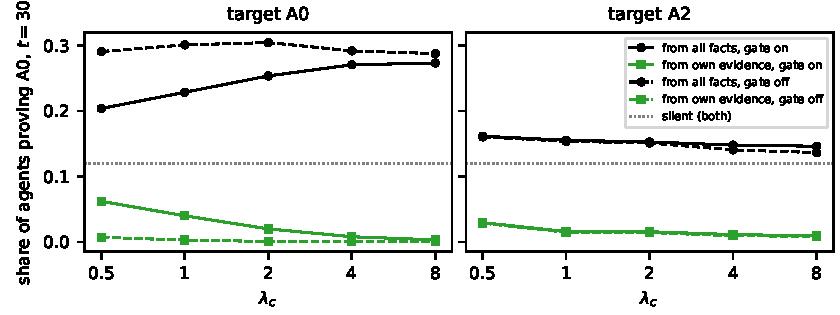
\includegraphics[width=0.66\linewidth]{figures/fig_own_proof.pdf}
\caption{Share of agents whose memory proves A0 at $t = 30$: from all their facts (black) and
from the agents' original facts only (green); dotted: silent swarm.}
\label{fig:ownproof}
\end{figure}

Without a controller, 12\% of agents prove A0 at $t = 30$, all from the agents' own facts.
The truth controller raises the share proving A0 to 20--30\%, but the share proving it
\emph{from the agents' own facts} falls to 6\% (slow, gated controller) and to almost 0 when
it posts more (Figure~\ref{fig:ownproof}). Agents posting a controller fact do not post their
own, so their own evidence circulates less. The false controller, whose facts are also
true, raises proofs of A0 too (to 14--16\%) while own-evidence proofs fall to 1--3\%.
Simulation 1 showed the same substitution.

\section{The controller overestimates its support}

\begin{figure}[H]
\centering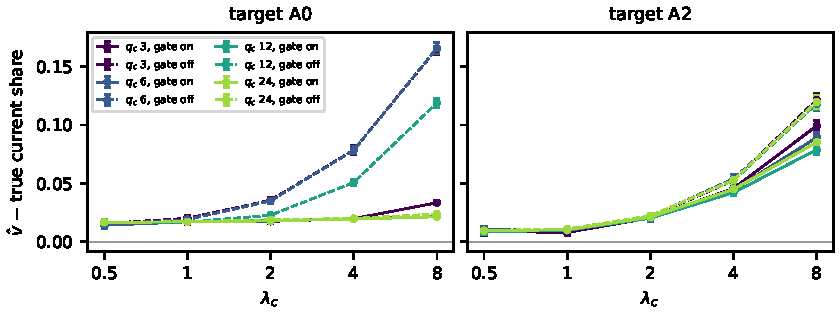
\includegraphics[width=0.66\linewidth]{figures/fig_sensing.pdf}
\caption{Error of the controller's estimate $\hat v$ (share of posts read whose author voted
for the target) against the true current share of all 24 agents' last votes; solid gate on,
dashed off.}
\label{fig:sensing}
\end{figure}

Unlike in Simulation 1, $\hat v$ is biased upward, and \textbf{the faster the controller, the
larger the bias}: about $+0.014$ at $\lambda_c \le 1$, rising to $+0.05$ (gate on) and $+0.14$
(gate off) at $\lambda_c = 8$. A likely reason, not yet tested: the posts it reads come from agents who
acted recently, often just after reading the controller's facts, while the true share also
counts older votes. More posts read ($q_c$) reduce the error's spread but not the bias.

\paragraph{Caveats.} One world (task\_003), 24 agents, exact-Bayesian agents,
probability-matching votes; a controller without memory that posts one fact at a time; a
budget of 30 messages. Means over 1{,}000 episodes per setting. Full analysis, code and
tables: \texttt{analysis/task003\_llm\_free/simulation\_2/analysis/} (report of 9 October,
reviewer guide).

\end{document}
